\section{Evaluation on Different Analysis Tasks} \label{sec:analysis-tasks}

\begin{table}[b]
  \centering
  % \begin{tabular}{p{0.08\textwidth}p{0.25\textwidth}p{0.12\textwidth}}
	\begin{tabular}{l l l}
  \toprule
  Name & Type & Data type \\
  \midrule
  boiler~\cite{boiler} & combustion simulation& float64\\
  plasma~\cite{magnetic} & magnetic reconnection simulation& float32\\
  diffusivity~\cite{cook_cabot_miller_2004} & hydrodynamics simulation& float64\\
  pressure~\cite{cook_cabot_miller_2004} & hydrodynamics simulation& float64\\
	turbulence~\cite{turbulence} & fluid dynamics simulation& float32\\
	kingsnake~\cite{kingsnake} & CT scan & uint8\\
	foam & CT scan & uint16\\
  \bottomrule
  \end{tabular}\label{tbl:data-sets}
  \vspace{-0.5em}
   \caption{Data sets used in our experiments; all volumes are $64^3$. Additional data sets are 
   included in the supplementary material.}
\end{table}

Thus far, we have presented several types of streams: data-independent (\slvl, \sbit, \swav),
data-dependent and task-independent (\smag), and task-dependent (\sopt, \ssig). In this section, we
consider a variety of common analysis and visualization tasks to evaluate the performance of these
streams. For each task, we define an error metric, $\err$, for the evaluation and comparison of
streams. Using \Cref{alg:greedy}, we compute streams specifically optimized for each task, \stkop,
and use its signature to compute the corresponding \stksg. For a variety of data sets, we compare
these streams by evaluating the error as a function of bits per samples (or \emph{bps}), defined as
the total number of bits received divided by the total number of samples. To mimic the effects of
entropy compression commonly used in practice, we remove from each stream all packets that consist
only of leading-zero bits. The wavelet basis allows us to always reconstruct data at full
resolution, which greatly simplifies computation of errors, as there exists no standard method to
compute error between grids of different dimensions.

\subsection{Function Reconstruction}\label{sec:rmse-optimized}

\begin{figure*}[t]
\centering
\subcaptionbox{\emph{boiler}}{%
{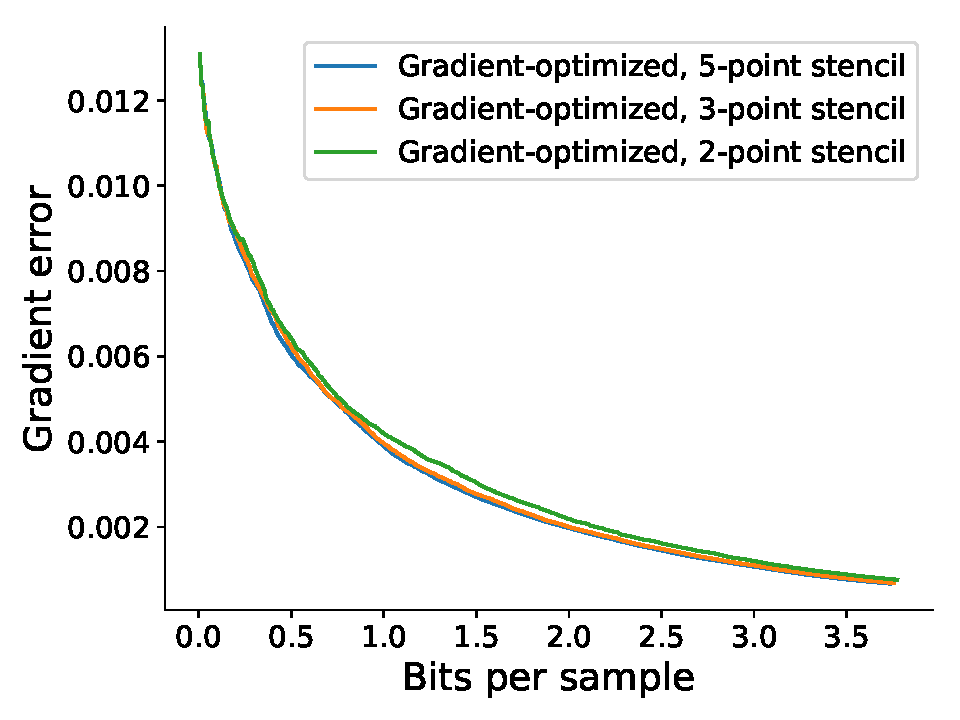
\includegraphics[width=0.24\linewidth]{gradient/gradient-optimized-boiler}}}
\subcaptionbox{\emph{diffusivity}}{%
{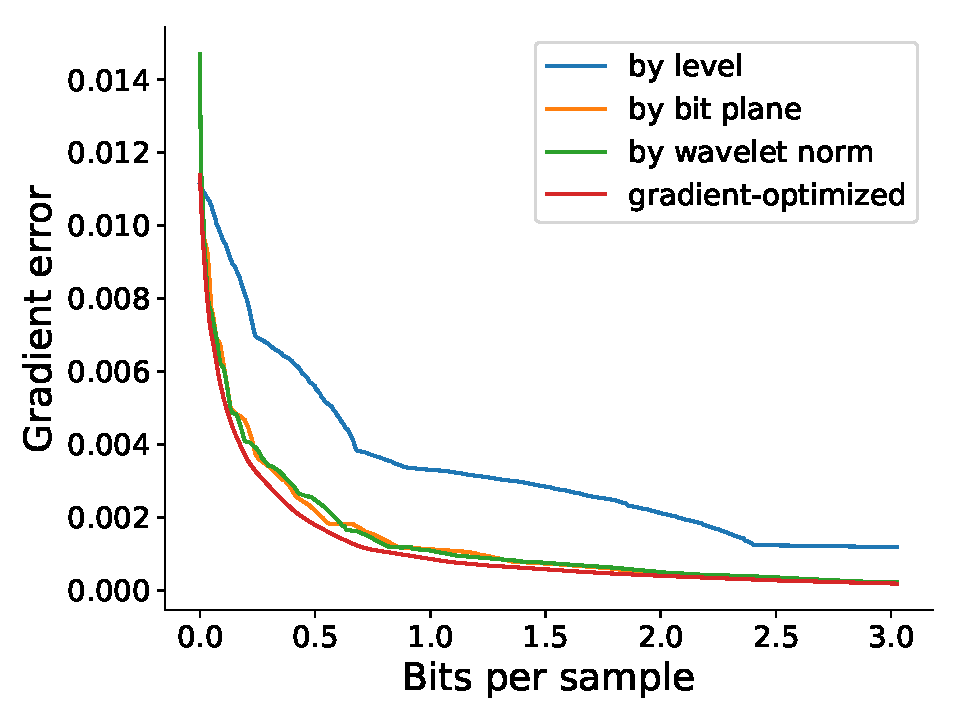
\includegraphics[width=0.24\linewidth]{gradient/gradient-optimized-diffusivity}}}
\subcaptionbox{\emph{turbulence}}{%
{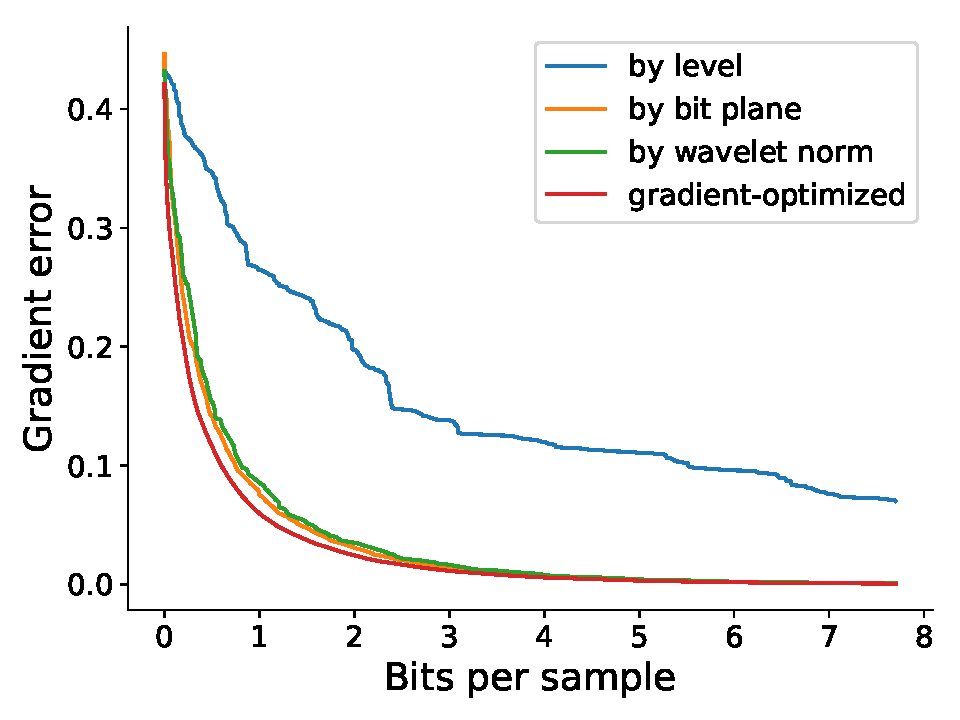
\includegraphics[width=0.24\linewidth]{gradient/gradient-optimized-turbulence}}}
\subcaptionbox{\emph{pressure}}{%
{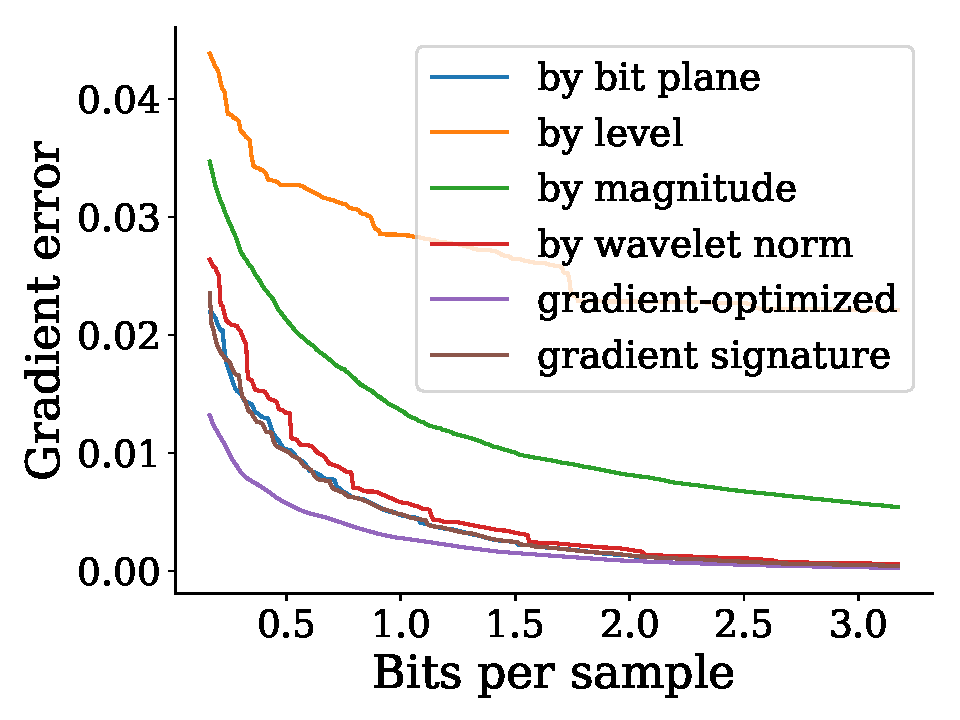
\includegraphics[width=0.24\linewidth]{gradient/gradient-optimized-pressure}}} 
\caption{Gradient error of reconstructed functions. Lower gradient error is better. Leading zero
packets are removed, and the plots are truncated in the same way as in~\Cref{fig:rmse-optimized}.
The trend in error, in all cases, is $\sgop < \sgsg \approx \sbit \approx \swav < \smag < \slvl$.}
\label{fig:gradient-error-comparison}
\vspace{1em}

\centering
\subcaptionbox{\emph{by level} (\slvl)}{%
{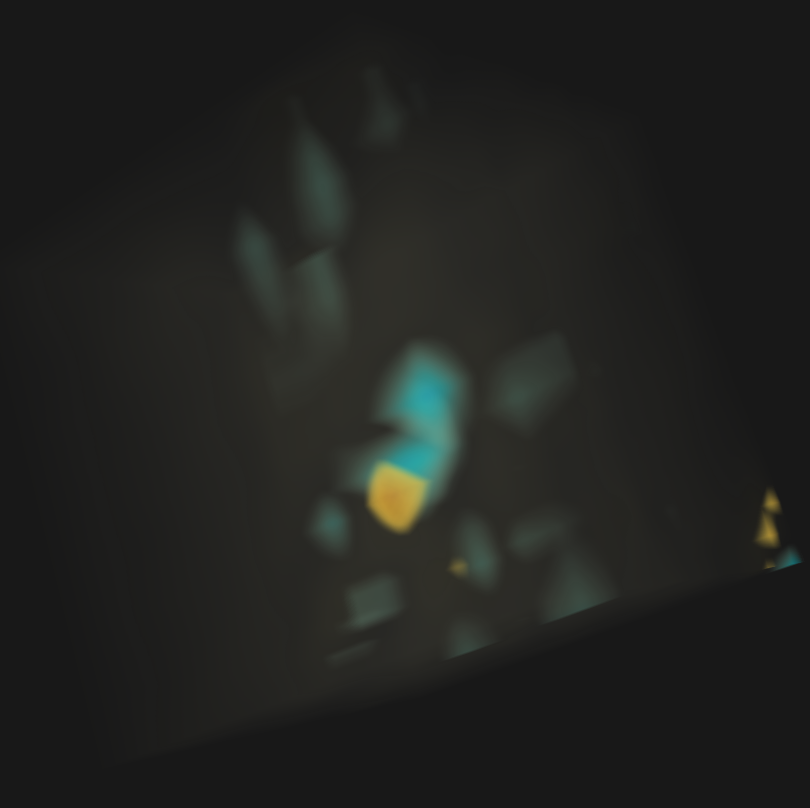
\includegraphics[width=0.16\linewidth]{gradient/gradient-turbulence-level}}}
\subcaptionbox{\emph{by bit plane} (\sbit)}{%
{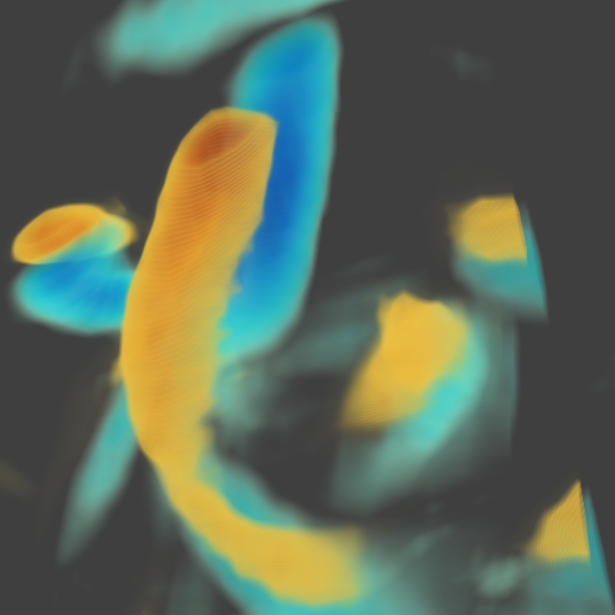
\includegraphics[width=0.16\linewidth]{gradient/gradient-turbulence-bit-plane}}}
\subcaptionbox{\emph{by wavelet norm} (\swav)}{%
{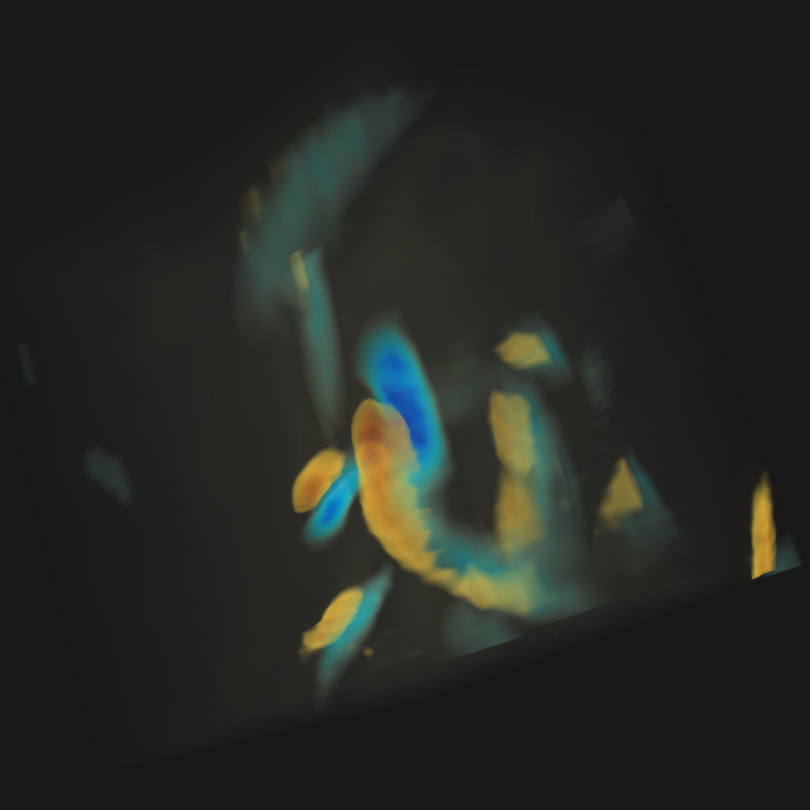
\includegraphics[width=0.16\linewidth]{gradient/gradient-turbulence-wavelet-norm}}}
\subcaptionbox{\emph{by magnitude} (\smag)}{%
{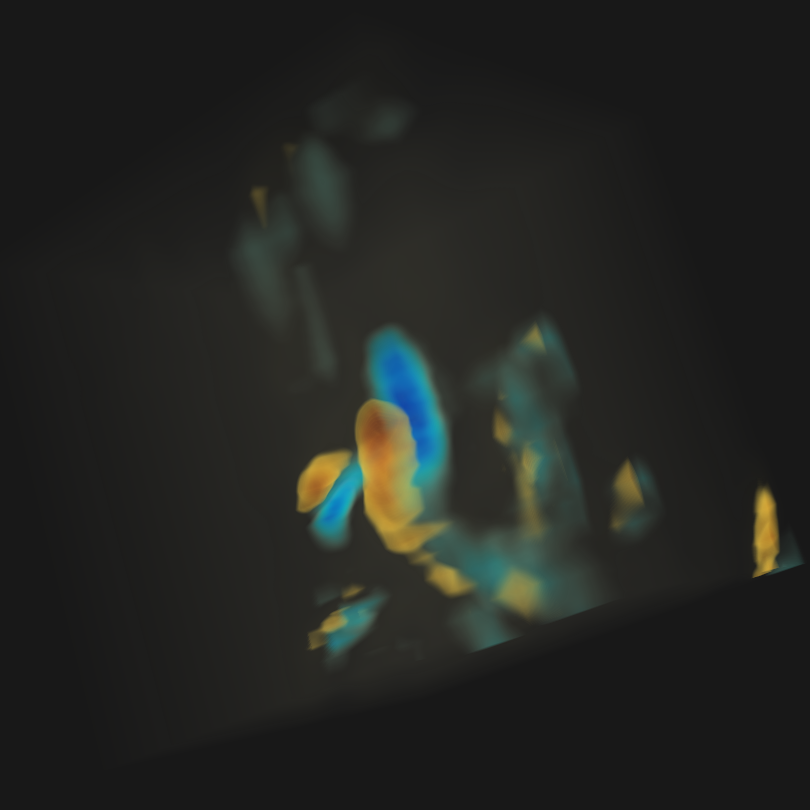
\includegraphics[width=0.16\linewidth]{gradient/gradient-turbulence-magnitude}}}
\subcaptionbox{\emph{by signature} (\sgsg)}{%
{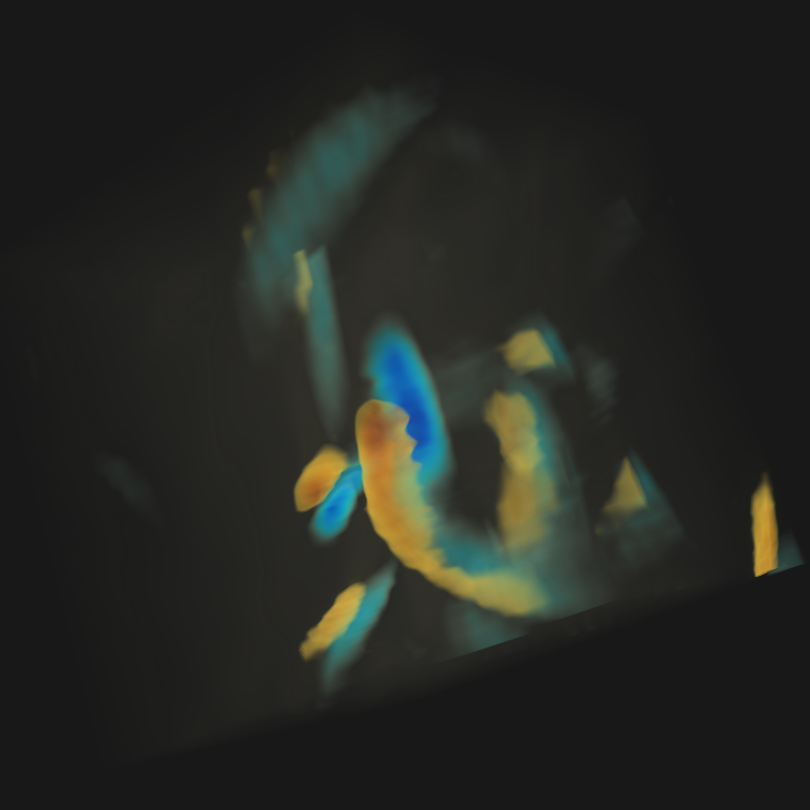
\includegraphics[width=0.16\linewidth]{gradient/gradient-turbulence-signature.png}}}
\subcaptionbox{\emph{reference}}{%
{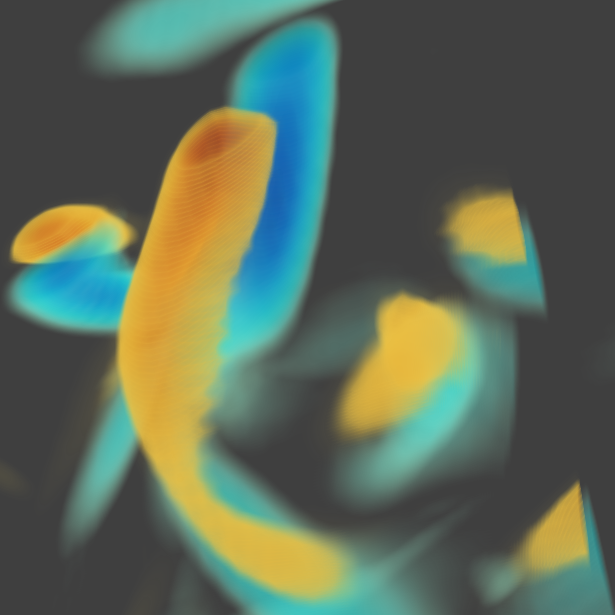
\includegraphics[width=0.16\linewidth]{gradient/gradient-turbulence-groundtruth.png}}}
\caption{The $x$-component of the ($64^3$) gradient field of \emph{turbulence}, reconstructed at 0.3
bps. The gradient field produced by \sbit is more accurate than the one produced by \swav, and
slightly more accurate than the one produced by \sgsg (compare orange features).}
\label{fig:gradient-rendering-diff}
\vspace{-1em}
\end{figure*}

One of the most fundamental analysis tasks is that of reconstructing the original function itself. A
commonly used error metric in this case is the root-mean-square error
(RMSE).~\Cref{fig:rmse-optimized} shows a comparison of the different streams for a variety of data
sets. It can be noted that, in general, \srop (the stream optimized to minimize the RMSE) performs
better than \srsg due to spatial adaptivity, whereas \srsg slightly outperforms \swav, followed by
\sbit, \smag, and \slvl.

In particular, \sbit outperforms \slvl (for \emph{kingsnake} and \emph{boiler}, it does so after
approximately 1 bps), which can be attributed to the removal of leading-zero packets. Empirically,
wavelet coefficients on finer scale subbands are much smaller in magnitude~\cite{spiht1996}. Such
coefficients contain a majority of the leading-zero bits, whose removal benefits \sbit the most.
\emph{diffusivity} and \emph{plasma} contain a significant amount of empty space, which translates
to more leading-zero bits after the wavelet transform that \sbit can take advantage of. This is the
reason why, unlike for \emph{boiler} and \emph{kingsnake}, \sbit outperforms \slvl immediately from
the beginning for \emph{diffusivity} and \emph{plasma}.

\smag underperforms for the same reason that \slvl does, but to a lesser extent, since \smag is
better adapted to the data. \swav outperforms both \slvl and \sbit, because it follows the optimal
(data-independent) bit ordering in $\Sigma_{L,B}$ in the $L_2$ norm, which is also the norm that
RMSE is based upon. Unsurprisingly, \srop outperforms all the others, as it is the most
data-adaptive (i.e., it can prioritize packets in the spatial domain in addition to the
$\Sigma_{L,B}$ domain). \srsg is the second best stream, as it follows the bit ordering of \srop in
$\Sigma_{L,B}$, but lacks any spatial adaptivity. In general, \swav and \ssig have similar
performances, but \ssig performs better when the data is less smooth or noisy, as is the case for
\emph{boiler} and \emph{kingsnake}. For such data, fine-level packets tends to have very few leading
one bits among a majority of leading zero bits, which \swav does not take into account (this stream
in effect assumes every packet contains all one bits).

We explore the errors visually by rendering the \emph{plasma} volume at 0.2 bits per sample (bps),
for all streams except \srop ~(\Cref{fig:rmse-rendering}). Bps are calculated by dividing the total
size of received packets (in bits) by the total number of samples. Although \slvl has the precision
to obtain an accurate background, it lacks resolution to resolve the fine details. \sbit, instead,
lacks the precision to reconstruct the (mostly smooth) background, but has enough resolution to
capture the fine details well. \swav balances both precision and resolution, producing a more
accurate picture as a whole. In this case, the \ssig stream manages to produce the most accurate
rendering, likely due to the ``anisotropic'' nature of the data, where most features lie on a thin
``surface''. For such data, wavelet coefficients along one dimension are often larger compared to
those along other dimensions, which \srop, and hence \srsg, can take advantage of, but not \swav.
